%%%%%%%%%%%%%%%%%%%%%%%%%%%%%%%%%%%%%%%%%%%%%%%%%%%
%% LaTeX book template                           %%
%% Author:  Amber Jain (http://amberj.devio.us/) %%
%% License: ISC license                          %%
%%%%%%%%%%%%%%%%%%%%%%%%%%%%%%%%%%%%%%%%%%%%%%%%%%%

\documentclass[a4paper,11pt]{book}
\usepackage[T1]{fontenc}
\usepackage[utf8]{inputenc}
\usepackage{lmodern}
%%%%%%%%%%%%%%%%%%%%%%%%%%%%%%%%%%%%%%%%%%%%%%%%%%%%%%%%%
% Source: http://en.wikibooks.org/wiki/LaTeX/Hyperlinks %
%%%%%%%%%%%%%%%%%%%%%%%%%%%%%%%%%%%%%%%%%%%%%%%%%%%%%%%%%
\usepackage{hyperref}
\usepackage[english]{babel}
% raaz commented these
%\usepackage{graphicx}
% raaz added these
\usepackage[pdftex]{graphicx}
\usepackage[final]{pdfpages}
\usepackage{pgfplots}
\usepackage{rotating}
\usepackage{amsmath,amssymb}
\usepackage{wrapfig}
\usepackage{intmacros}% raaz's notation for interval, random, set-valued objects in one notation
%%%% avoiding ps
%\usepackage{pstricks}
%\usepackage{pst-plot}
%\usepackage[pdf]{pstricks}

%%%%%%%%%%%%%%%%%%%%%%%%%%%%%%%%%%%%%%%%%%%%%%%%%%%%%%%%%%%%%%%%%%%%%%%%%%%%%%%%
% 'dedication' environment: To add a dedication paragraph at the start of book %
% Source: http://www.tug.org/pipermail/texhax/2010-June/015184.html            %
%%%%%%%%%%%%%%%%%%%%%%%%%%%%%%%%%%%%%%%%%%%%%%%%%%%%%%%%%%%%%%%%%%%%%%%%%%%%%%%%
\newenvironment{dedication}
{
   \cleardoublepage
   \thispagestyle{empty}
   \vspace*{\stretch{1}}
   \hfill\begin{minipage}[t]{0.66\textwidth}
   \raggedright
}
{
   \end{minipage}
   \vspace*{\stretch{3}}
   \clearpage
}

%%%%%%%%%%%%%%%%%%%%%%%%%%%%%%%%%%%%%%%%%%%%%%%%
% Chapter quote at the start of chapter        %
% Source: http://tex.stackexchange.com/a/53380 %
%%%%%%%%%%%%%%%%%%%%%%%%%%%%%%%%%%%%%%%%%%%%%%%%
\makeatletter
\renewcommand{\@chapapp}{}% Not necessary...
\newenvironment{chapquote}[2][2em]
  {\setlength{\@tempdima}{#1}%
   \def\chapquote@author{#2}%
   \parshape 1 \@tempdima \dimexpr\textwidth-2\@tempdima\relax%
   \itshape}
  {\par\normalfont\hfill--\ \chapquote@author\hspace*{\@tempdima}\par\bigskip}
\makeatother

%%%%%%%%%%%%%%%%%%%%%%%%%%%%%%%%%%%%%%%%%%%%%%%%%%%
% First page of book which contains 'stuff' like: %
%  - Book title, subtitle                         %
%  - Book author name                             %
%%%%%%%%%%%%%%%%%%%%%%%%%%%%%%%%%%%%%%%%%%%%%%%%%%%

% Book's title and subtitle
\title{\Huge \textbf{Lectures by Jan-Erik Bj\"ork}  \footnote{Stockholm, Sweden, July--August 2016.} \\ \huge Constructive Elements of Geometry, Calculus, Solid Mechanics, Linear Algebra and Measures for Engineers and Statisticians  \footnote{scribed by Raazesh Sainudiin.}}
% Author
\author{\textsc{Jan-Erik Bj\"ork and Raazesh Sainudiin}\thanks{\url{http://corcon.net/about/}}}


\begin{document}

\frontmatter
\maketitle

%%%%%%%%%%%%%%%%%%%%%%%%%%%%%%%%%%%%%%%%%%%%%%%%%%%%%%%%%%%%%%%
% Add a dedication paragraph to dedicate your book to someone %
%%%%%%%%%%%%%%%%%%%%%%%%%%%%%%%%%%%%%%%%%%%%%%%%%%%%%%%%%%%%%%%
\begin{dedication}
Dedicated to Aristotle, Archimedes, Newton, Abel, Lagrange, Euler, ....
\end{dedication}

%%%%%%%%%%%%%%%%%%%%%%%%%%%%%%%%%%%%%%%%%%%%%%%%%%%%%%%%%%%%%%%%%%%%%%%%
% Auto-generated table of contents, list of figures and list of tables %
%%%%%%%%%%%%%%%%%%%%%%%%%%%%%%%%%%%%%%%%%%%%%%%%%%%%%%%%%%%%%%%%%%%%%%%%
\tableofcontents
\listoffigures
\listoftables

\mainmatter

%%%%%%%%%%%
% Preface %
%%%%%%%%%%%
\chapter*{Preface}
This is as set of face-to-face transmissions between Jan-Erik Bj\"ork and Raazesh Sainudiin on various topics related towards constructive elements of a machine-interval experiment involving a measurable double pendulum.

July--August, 2016\\
Stockholm, Sweden.

\noindent Jan-Erik Bj\"ork \& Raazesh Sainudiin \\
\noindent \url{http://www.math.canterbury.ac.nz/~r.sainudiin/index.shtml}
%\section*{Un-numbered sample section}

%\section*{Another sample section}

\section*{Structure of book}
% You might want to add short description about each chapter in this book.
Each unit will focus on a key idea.

%\section*{About the companion website}
%The website\footnote{\url{https://github.com/amberj/latex-book-template}} for this file contains:
%\begin{itemize}
%  \item A link to (freely downlodable) latest version of this document.
%  \item Link to download LaTeX source for this document.
%  \item Miscellaneous material (e.g. suggested readings etc).
%\end{itemize}

%%%%%%%%%%%%%%%%%%%%%%%%%%%%%%%%%%%%
% Give credit where credit is due. %
% Say thanks!                      %
%%%%%%%%%%%%%%%%%%%%%%%%%%%%%%%%%%%%
%\section*{Acknowledgements}
%\begin{itemize}
%\item A special word of thanks goes to Professor Don Knuth\footnote{\url{http://www-cs-faculty.stanford.edu/~uno/}} (for \TeX{}) and Leslie Lamport\footnote{\url{http://www.lamport.org/}} (for \LaTeX{}).
%\item I'll also like to thank Gummi\footnote{\url{http://gummi.midnightcoding.org/}} developers and LaTeXila\footnote{\url{http://projects.gnome.org/latexila/}} development team for their awesome \LaTeX{} editors.
%\item I'm deeply indebted my parents, colleagues and friends for their support and encouragement.
%\end{itemize}
%\mbox{}\\
%\mbox{}\\
%\noindent Amber Jain \\
%\noindent \url{http://amberj.devio.us/}

%%%%%%%%%%%%%%%%%%%%%%%%  BEGINNING OF CHAPTER %%%%%%%%%%%%%%%%%%%%%%%%%%%%%%%%

% examples of section, subsections and footnote
%\section{Section heading}
%\subsection{Lorem ipsum.}
%\noindent Lorem ipsum dolor siturna\footnote{Lorem ipsum lacus.}:
%imperdiet\footnote{\url{www.example.com}} erat

\chapter{Abel's Resolution of a Mechanical Problem}

\begin{chapquote}{Author's name, \textit{Source of this quote}}
``This is a quote and I don't know who said this.''
\end{chapquote}

\section{Abel's Resolution of a Mechanical Problem}

%see https://www.sharelatex.com/learn/Wrapping_text_around_figures
\begin{wrapfigure}{r}{0.5\textwidth}
\begin{center}
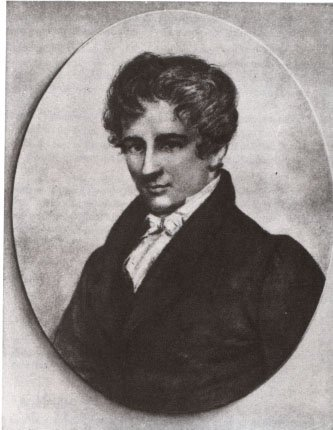
\includegraphics[width=0.25\textwidth]{figures/abel38968.jpg} 
\end{center}
\caption{Niels Henrik Abel}
\end{wrapfigure}
Niels Henrik Abel (1802-1829) was one of Norway's greatest mathematicians. 
He was born on August 5, 1802, in Frindoe, Norway, and died due to tuberculosis at the age of 26, on April 6, 1829 in Froland, Norway.\footnote{\url{http://turnbull.mcs.st-and.ac.uk/history/Biographies/Abel.html}}.

Here we focus on an empirically motivated inversion problem in his work titled {\em R\'esolution du'un probl\`eme de mechanique} (see scan in \ref{ORIGINALResolutionOfAMechanicalProblemByNielsHenrikAbel}) or {\em Resolution of a mechanical problem} that eventually leads to his elliptic integral\footnote{\url{http://www.maa.org/sites/default/files/images/upload_library/1/abeltranslation.pdf}}.

\section{Pippi's experiment in the fog}
\begin{figure}[htbp]
% see http://tex.stackexchange.com/questions/144454/how-to-plot-x1-3
\begin{center}
% set the arrows as stealth fighters
\tikzset{>=stealth}
\begin{tikzpicture}
  \begin{axis}[
xlabel={distance $x$}, ylabel={altitude $y$},
    xmin=-1,xmax=3,
    ymin=-1,ymax=1,
    axis lines=center,
    axis line style=<->]

%    \addplot[<->] expression[domain=-10:10,samples=100]{x/abs(x)*abs(x)^(1/3)}; 
    \addplot[<->] expression[domain=-1:1,samples=100]{0.5*x^(2)}; 
\addplot[mark=*] coordinates {(0,0)} node[pin=100:{puck}]{} ;
%\addplot[mark=.] coordinates {(0.25,0.125)} node[pin=20:{curve $u(x)$}]{} ;
\addplot[mark=.] coordinates {(0.75,0.28125)} node[pin=0:{curve $u(x)=y$}]{} ;
%\addplot[mark=.] coordinates {(0.75,0.649519052838329)} node[pin=100:{curve $u(x)$}]{} ;
  \end{axis}
\end{tikzpicture}
\end{center}
\end{figure}

\newpage

~\\
\newpage
~\\
\newpage


\section{Set up of Abel's original mechanical problem}\label{S:ORIGINALResolutionOfAMechanicalProblemByNielsHenrikAbel}

Let BDMA be any curve. BC is a horizontal line and CA a vertical line. 
Suppose that a point stressed by gravity moves on the curve, with any point D being the point of departure.  
Let $\tau$ be the time elapsed when the mobile point has reached the point A and let $a$ be the height EA.  
The quantity $\tau$ is some function of $a$, which depend on the form of the curve.
\begin{wrapfigure}{l}{0.5\textwidth}
\begin{center}
\begin{tabular}{c}
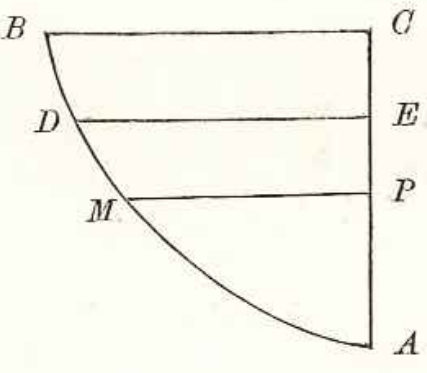
\includegraphics[width=0.4\textwidth]{figures/ResolutionOfAMechanicalProblemFig1.png}\\
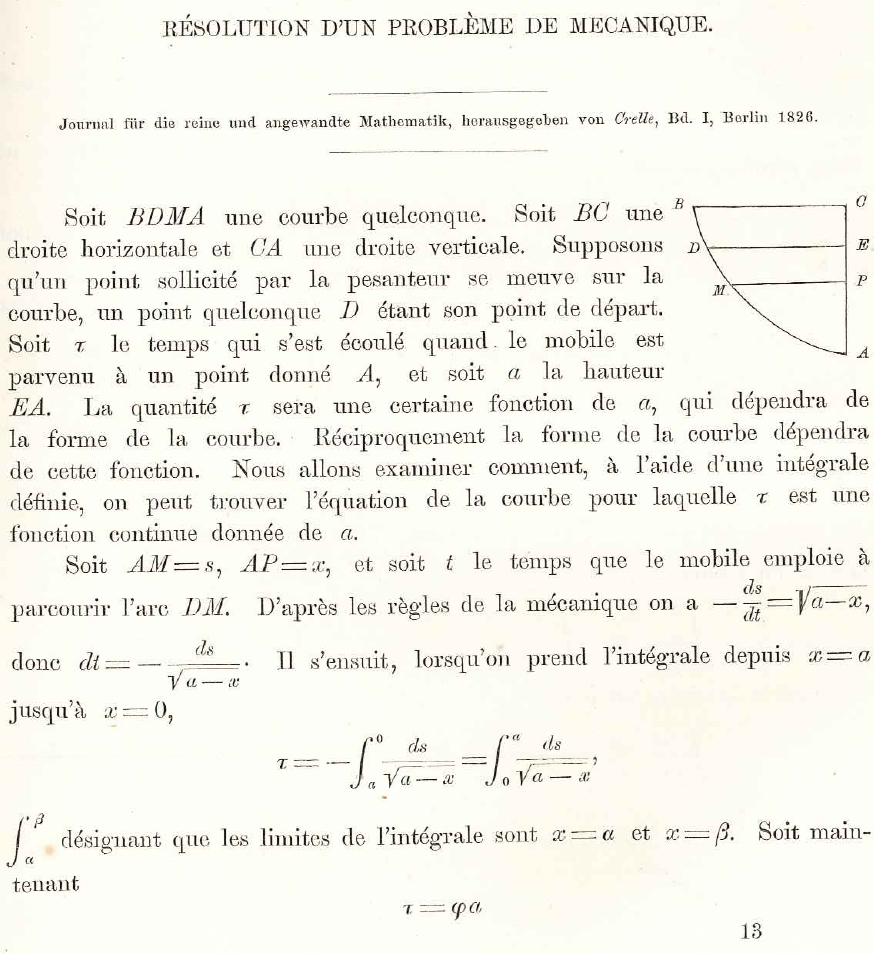
\includegraphics[width=0.4\textwidth,angle=0]{figures/ResolutionOfAMechanicalProblemPage1.png}\\
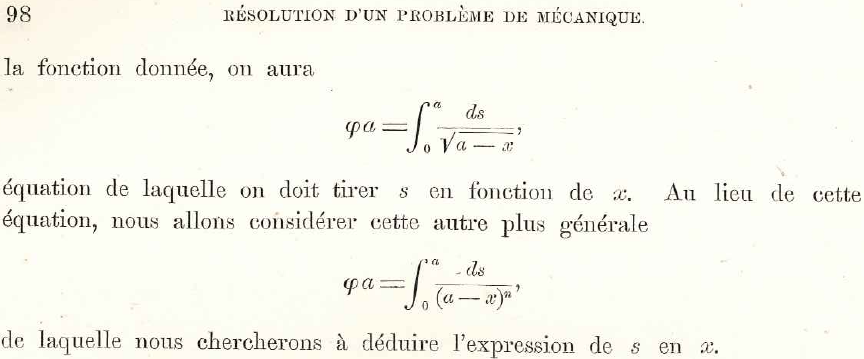
\includegraphics[width=0.4\textwidth,angle=0]{figures/ResolutionOfAMechanicalProblemPage2.png}
\end{tabular}
\end{center}
\caption{First two pages of {\em R\'esolution du'un probl\`eme de mechanique}}
\end{wrapfigure}
Conversely the form of the curve depends on this function.
We will examine how, with a definite integral, we can find the equation of the curve in which $\tau$ is a continuous function of given $a$.
Let $\mathrm{AM}=:s$, $\mathrm{AP}=:x$ and $t$ be the time that the mobile used to browse the arc $\mathrm{DM}$.  
According to the rules of mechanics:
\[
a-\frac{ds}{dt} = \sqrt{a-x}, \quad dt = - \frac{ds}{\sqrt{a-x}}
\]
It follows, when we take the integral from $x=a$ until $x=0$,
\[
\tau = - \int_{a}^{0} \frac{ds}{\sqrt{a-x}} = \int_{0}^{a} \frac{ds}{\sqrt{a-x}}
\]
$\int_{\alpha}^{\beta} \cdot$ designating the limits of the integral are $x=\alpha$ and $x=\beta$.  
Now maintaining
\[
\tau = \varphi a
\]
the given function, we will
\[
\varphi a = \int_0^{\alpha} \frac{ds}{\sqrt{a-x}} ,
\]
equation which we must draw $s$ as a function of $x$. ..
Instead of this equation, we consider the other more general
\[
\varphi a = \int_0^{\alpha} \frac{ds}{(a-x)^n} ,
\]
which we seek to deduce the expression of $s$ in $x$....

{\bf 
Legendre integral connection...
}

Next we provide a scan of the original work by Abel and make some remarks.

\newpage

%% later see
%see addtolist and addtotoc http://mirror.utexas.edu/ctan/macros/latex/contrib/pdfpages/pdfpages.pdf
%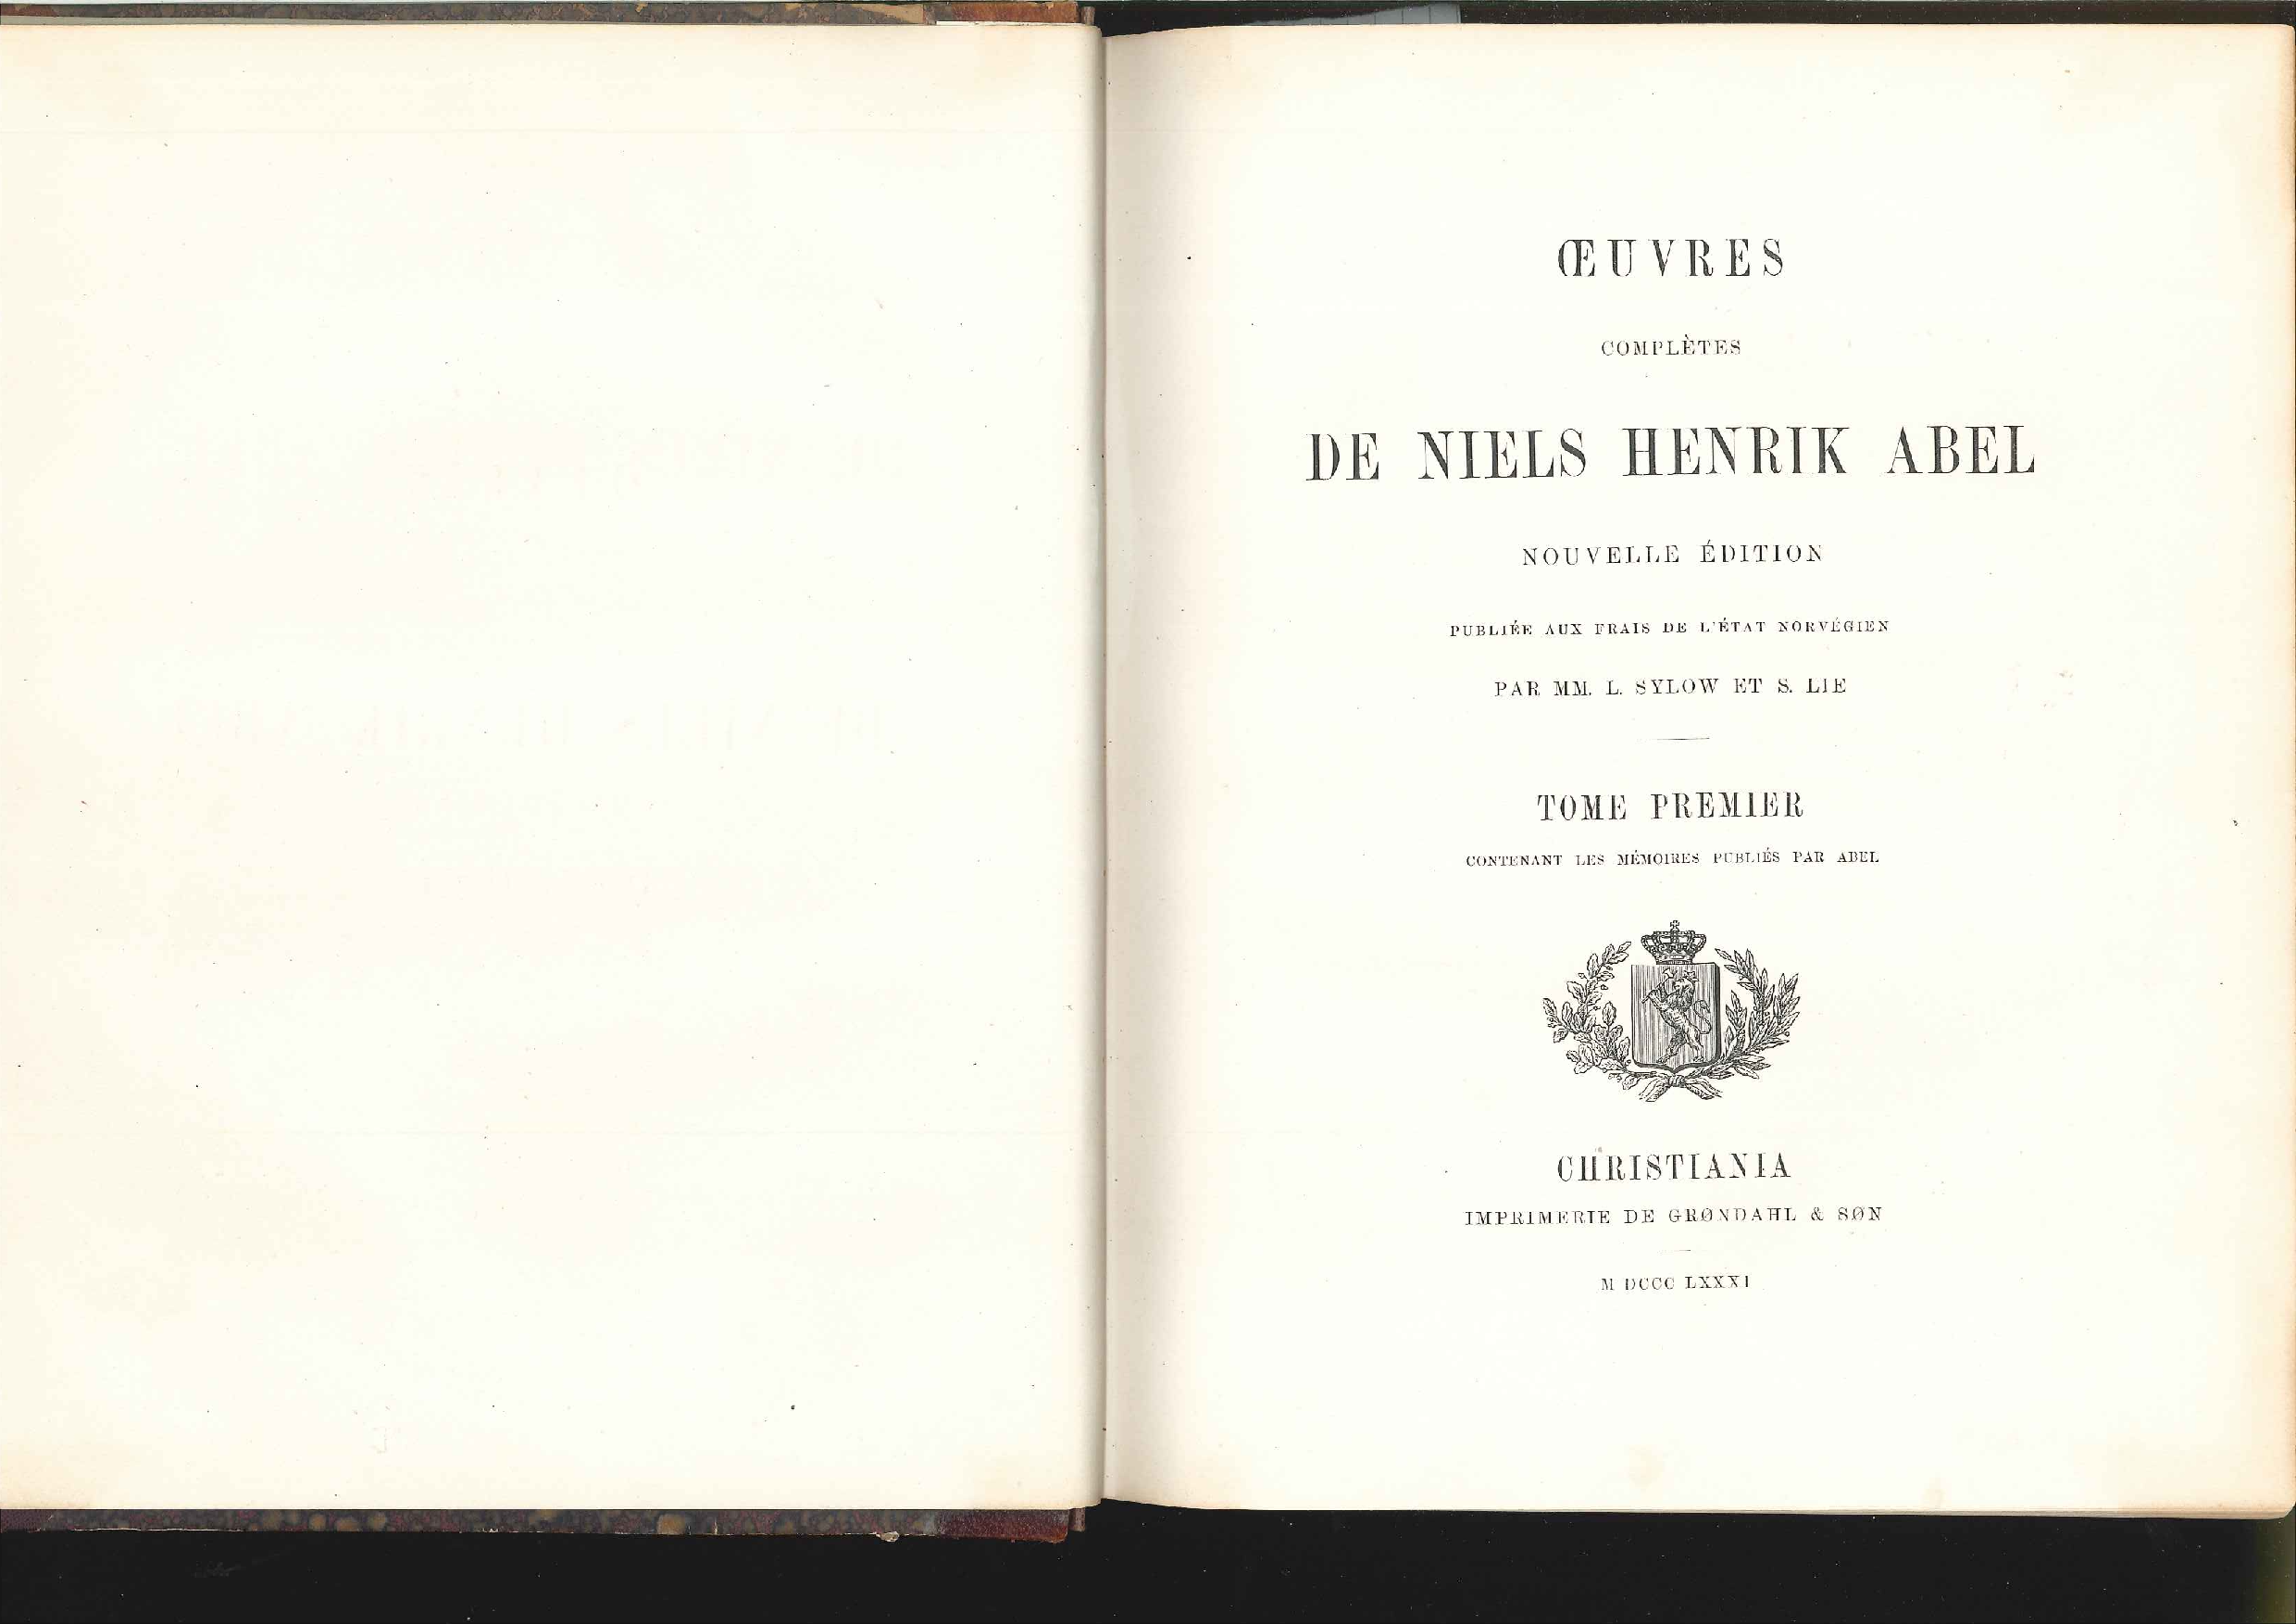
\includepdf[pages=-]{figures/20160720AbelTransformOriginal.pdf}
%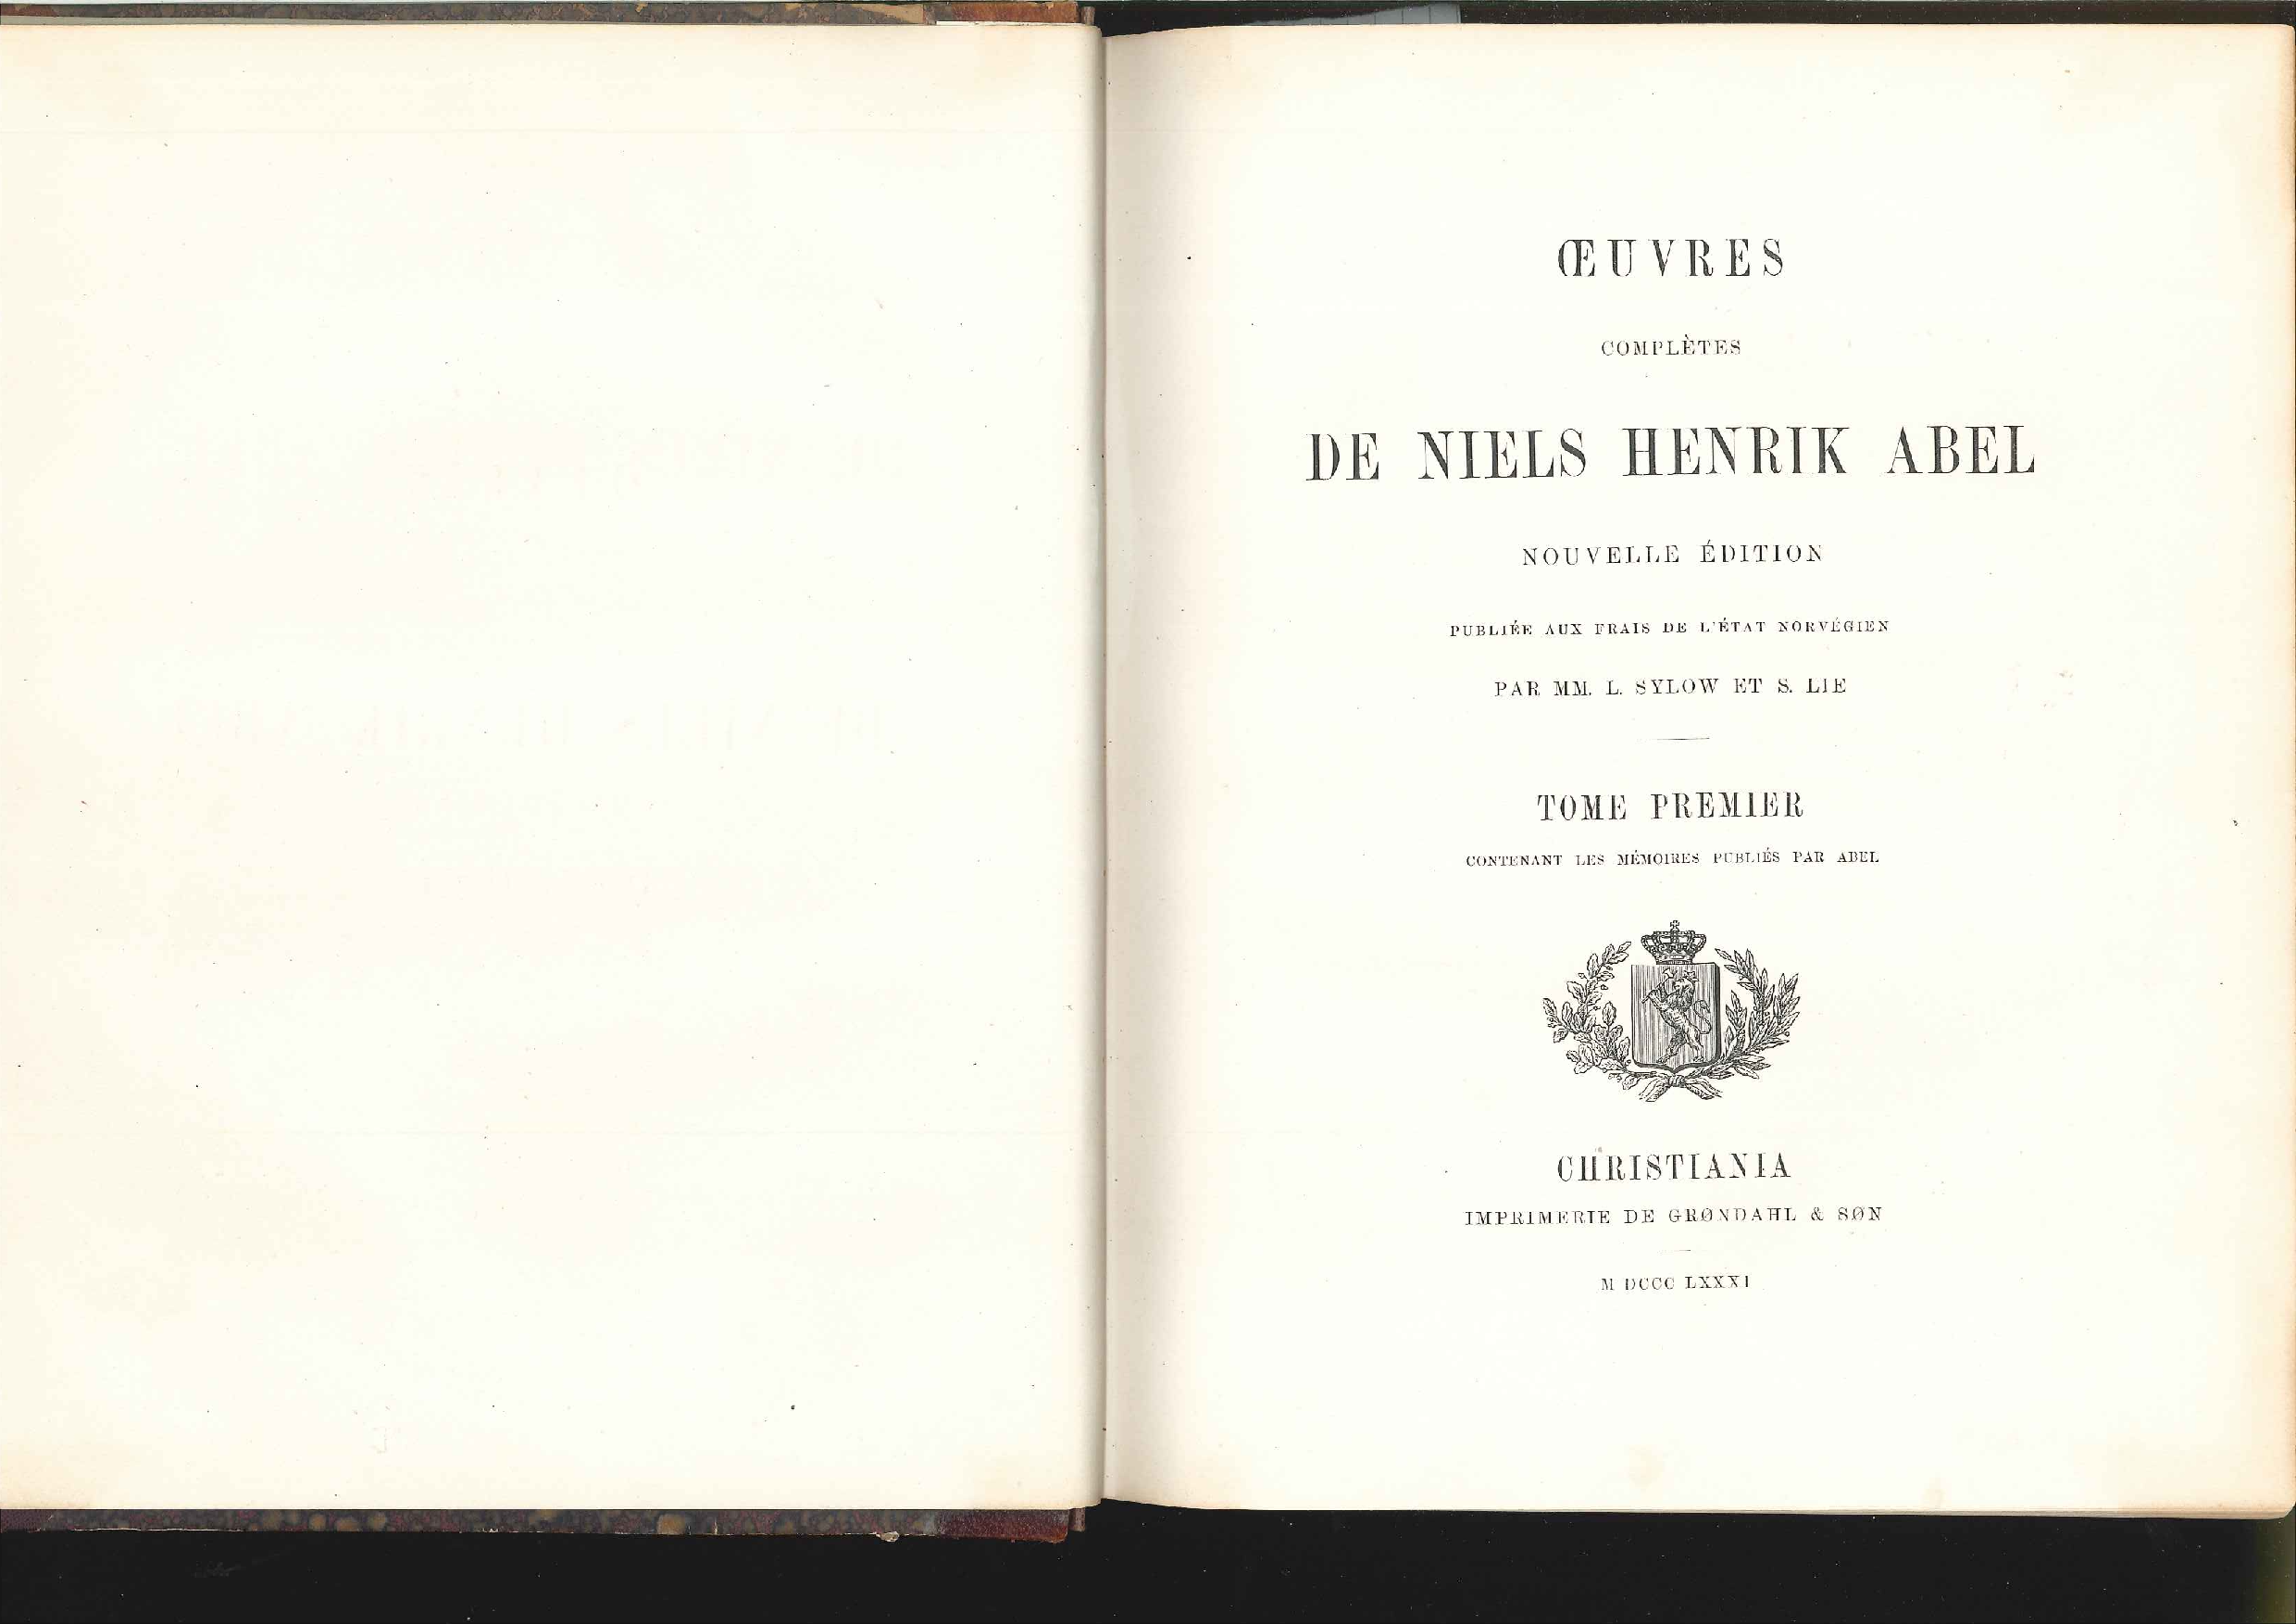
\includepdf[pages={1-4},nup=1x2,templatesize={145mm}{210mm},landscape=false,offset=0mm 0mm,delta=2mm 2mm]{figures/20160720AbelTransformOriginal.pdf}
%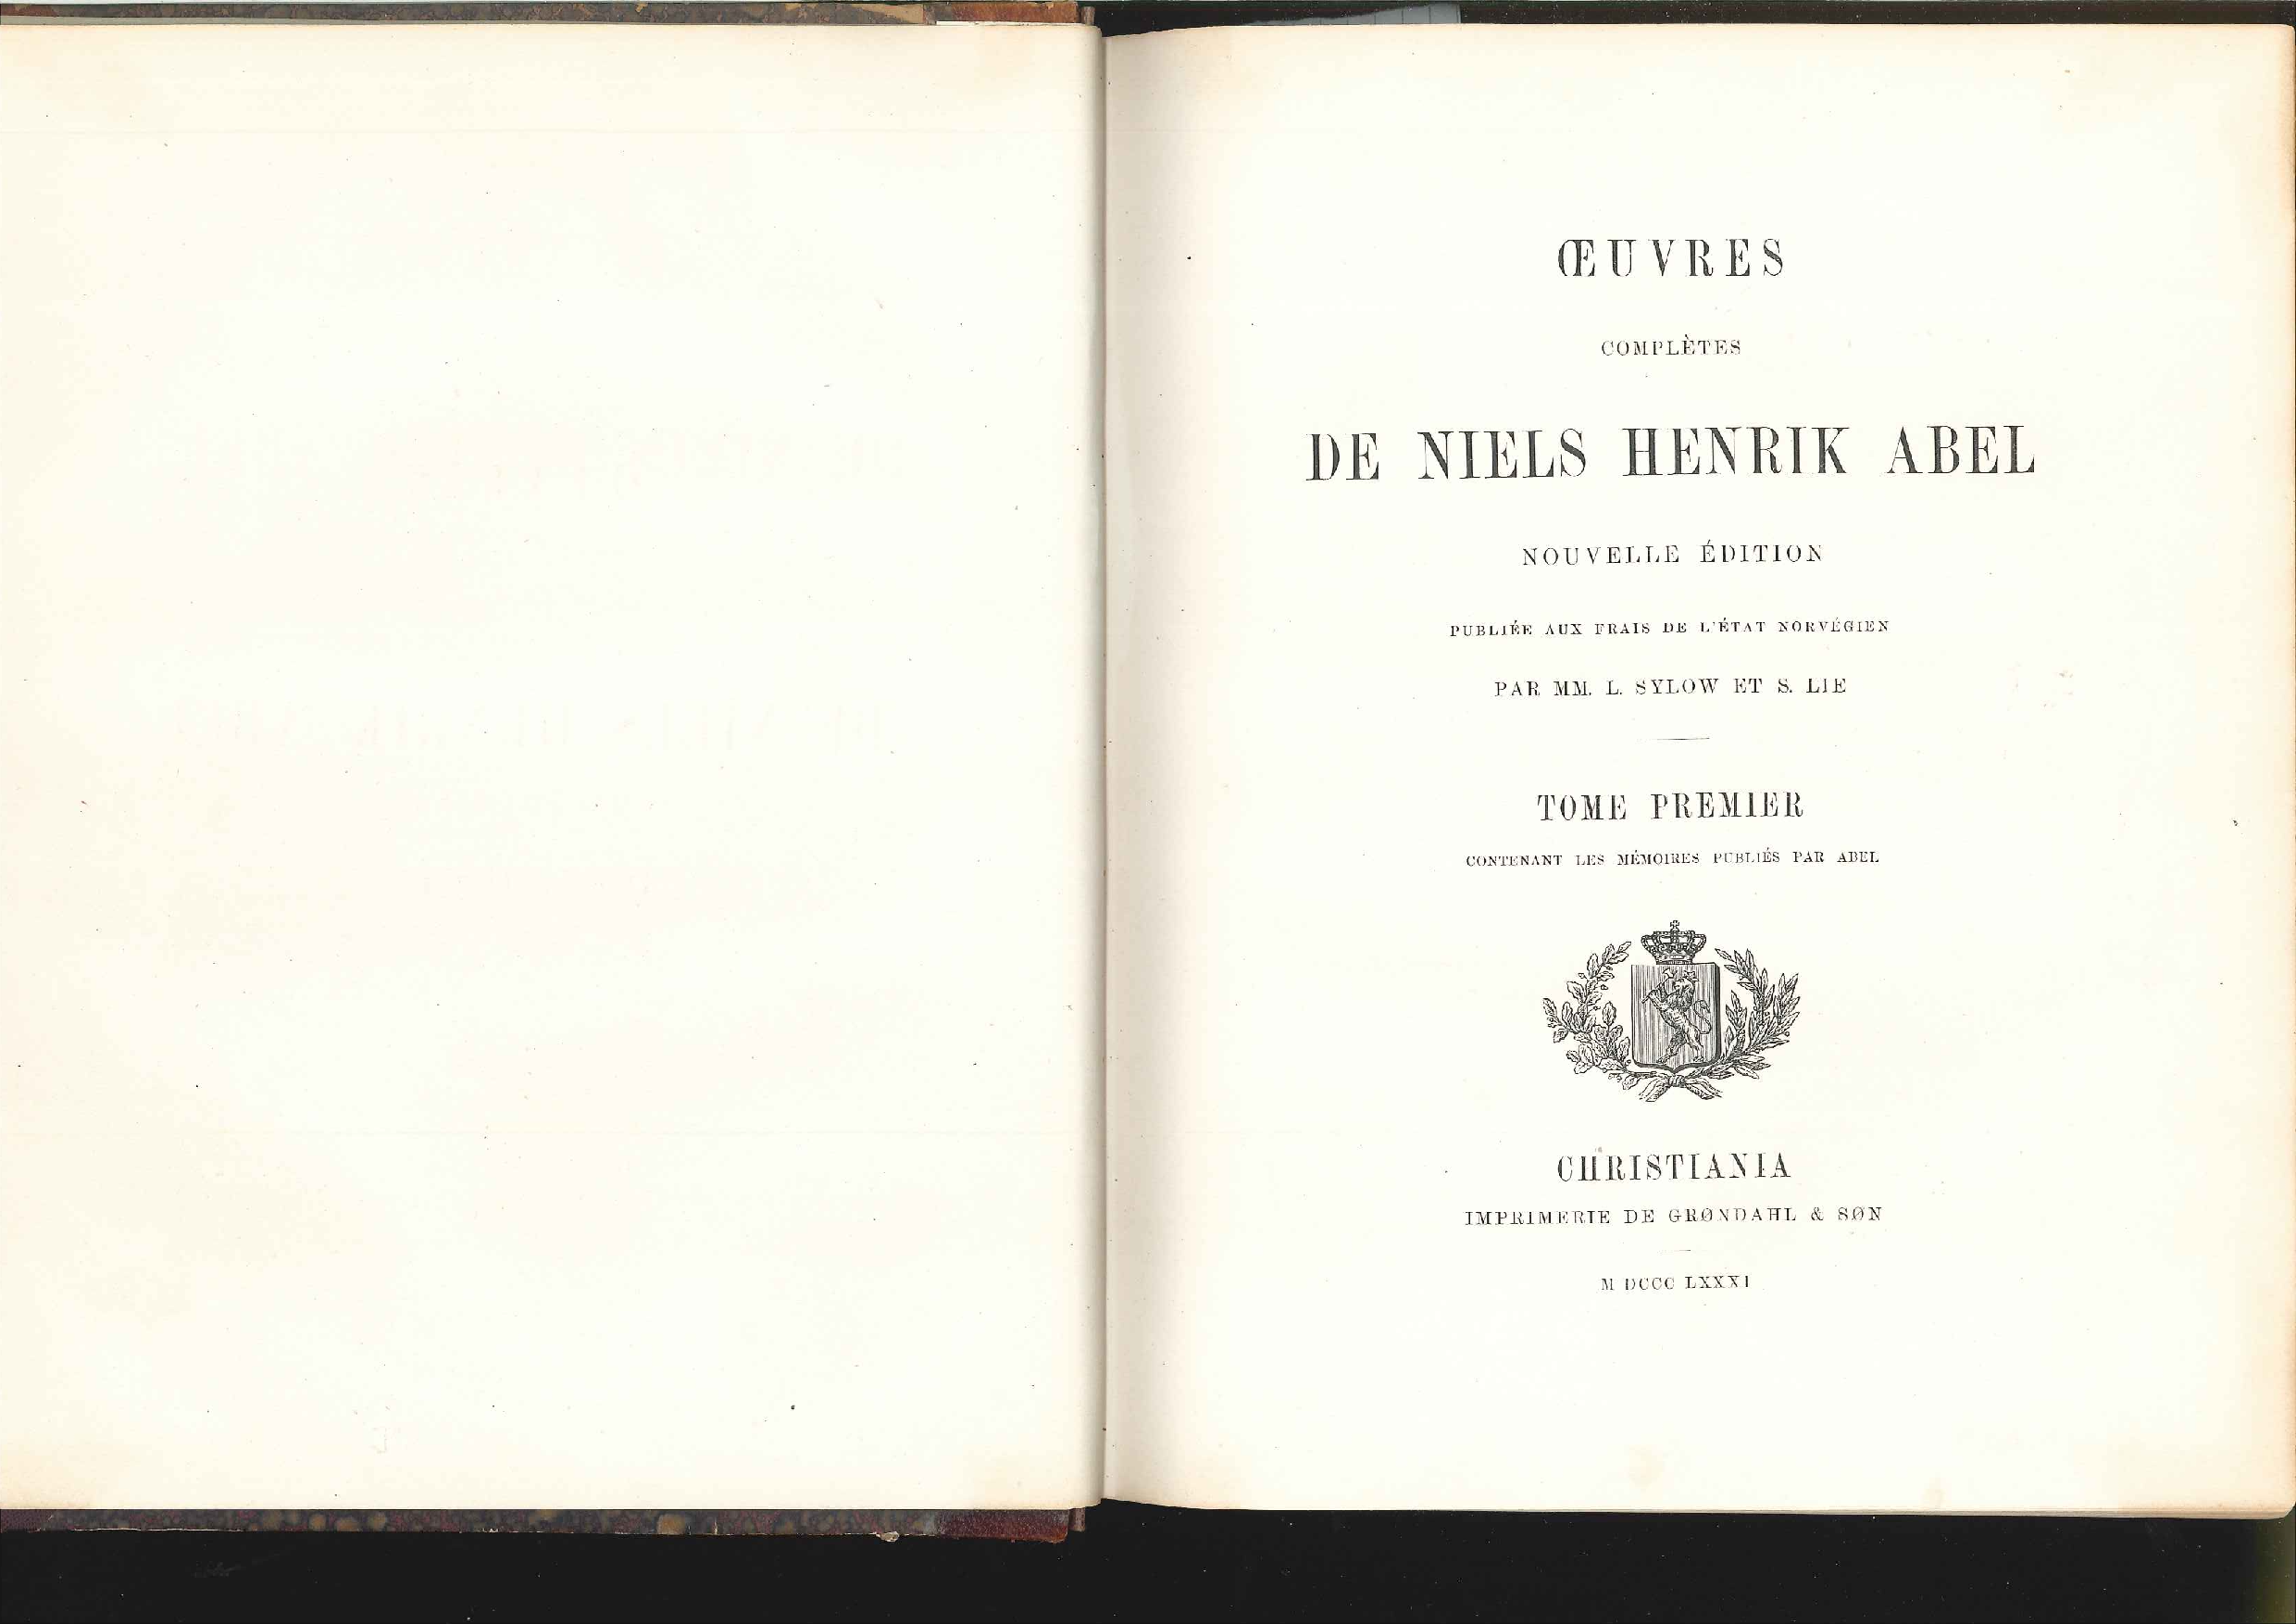
\includepdf[pages={1-4},nup=1x2,templatesize={\linewidth}{0.65\linewidth},landscape=false,offset=0mm 0mm,delta=2mm 2mm]{figures/20160720AbelTransformOriginal.pdf}
% see http://tex.stackexchange.com/questions/15989/toc-entries-and-labels-for-included-pdf-pages
%addtotoc={page number, section, level, heading, label}
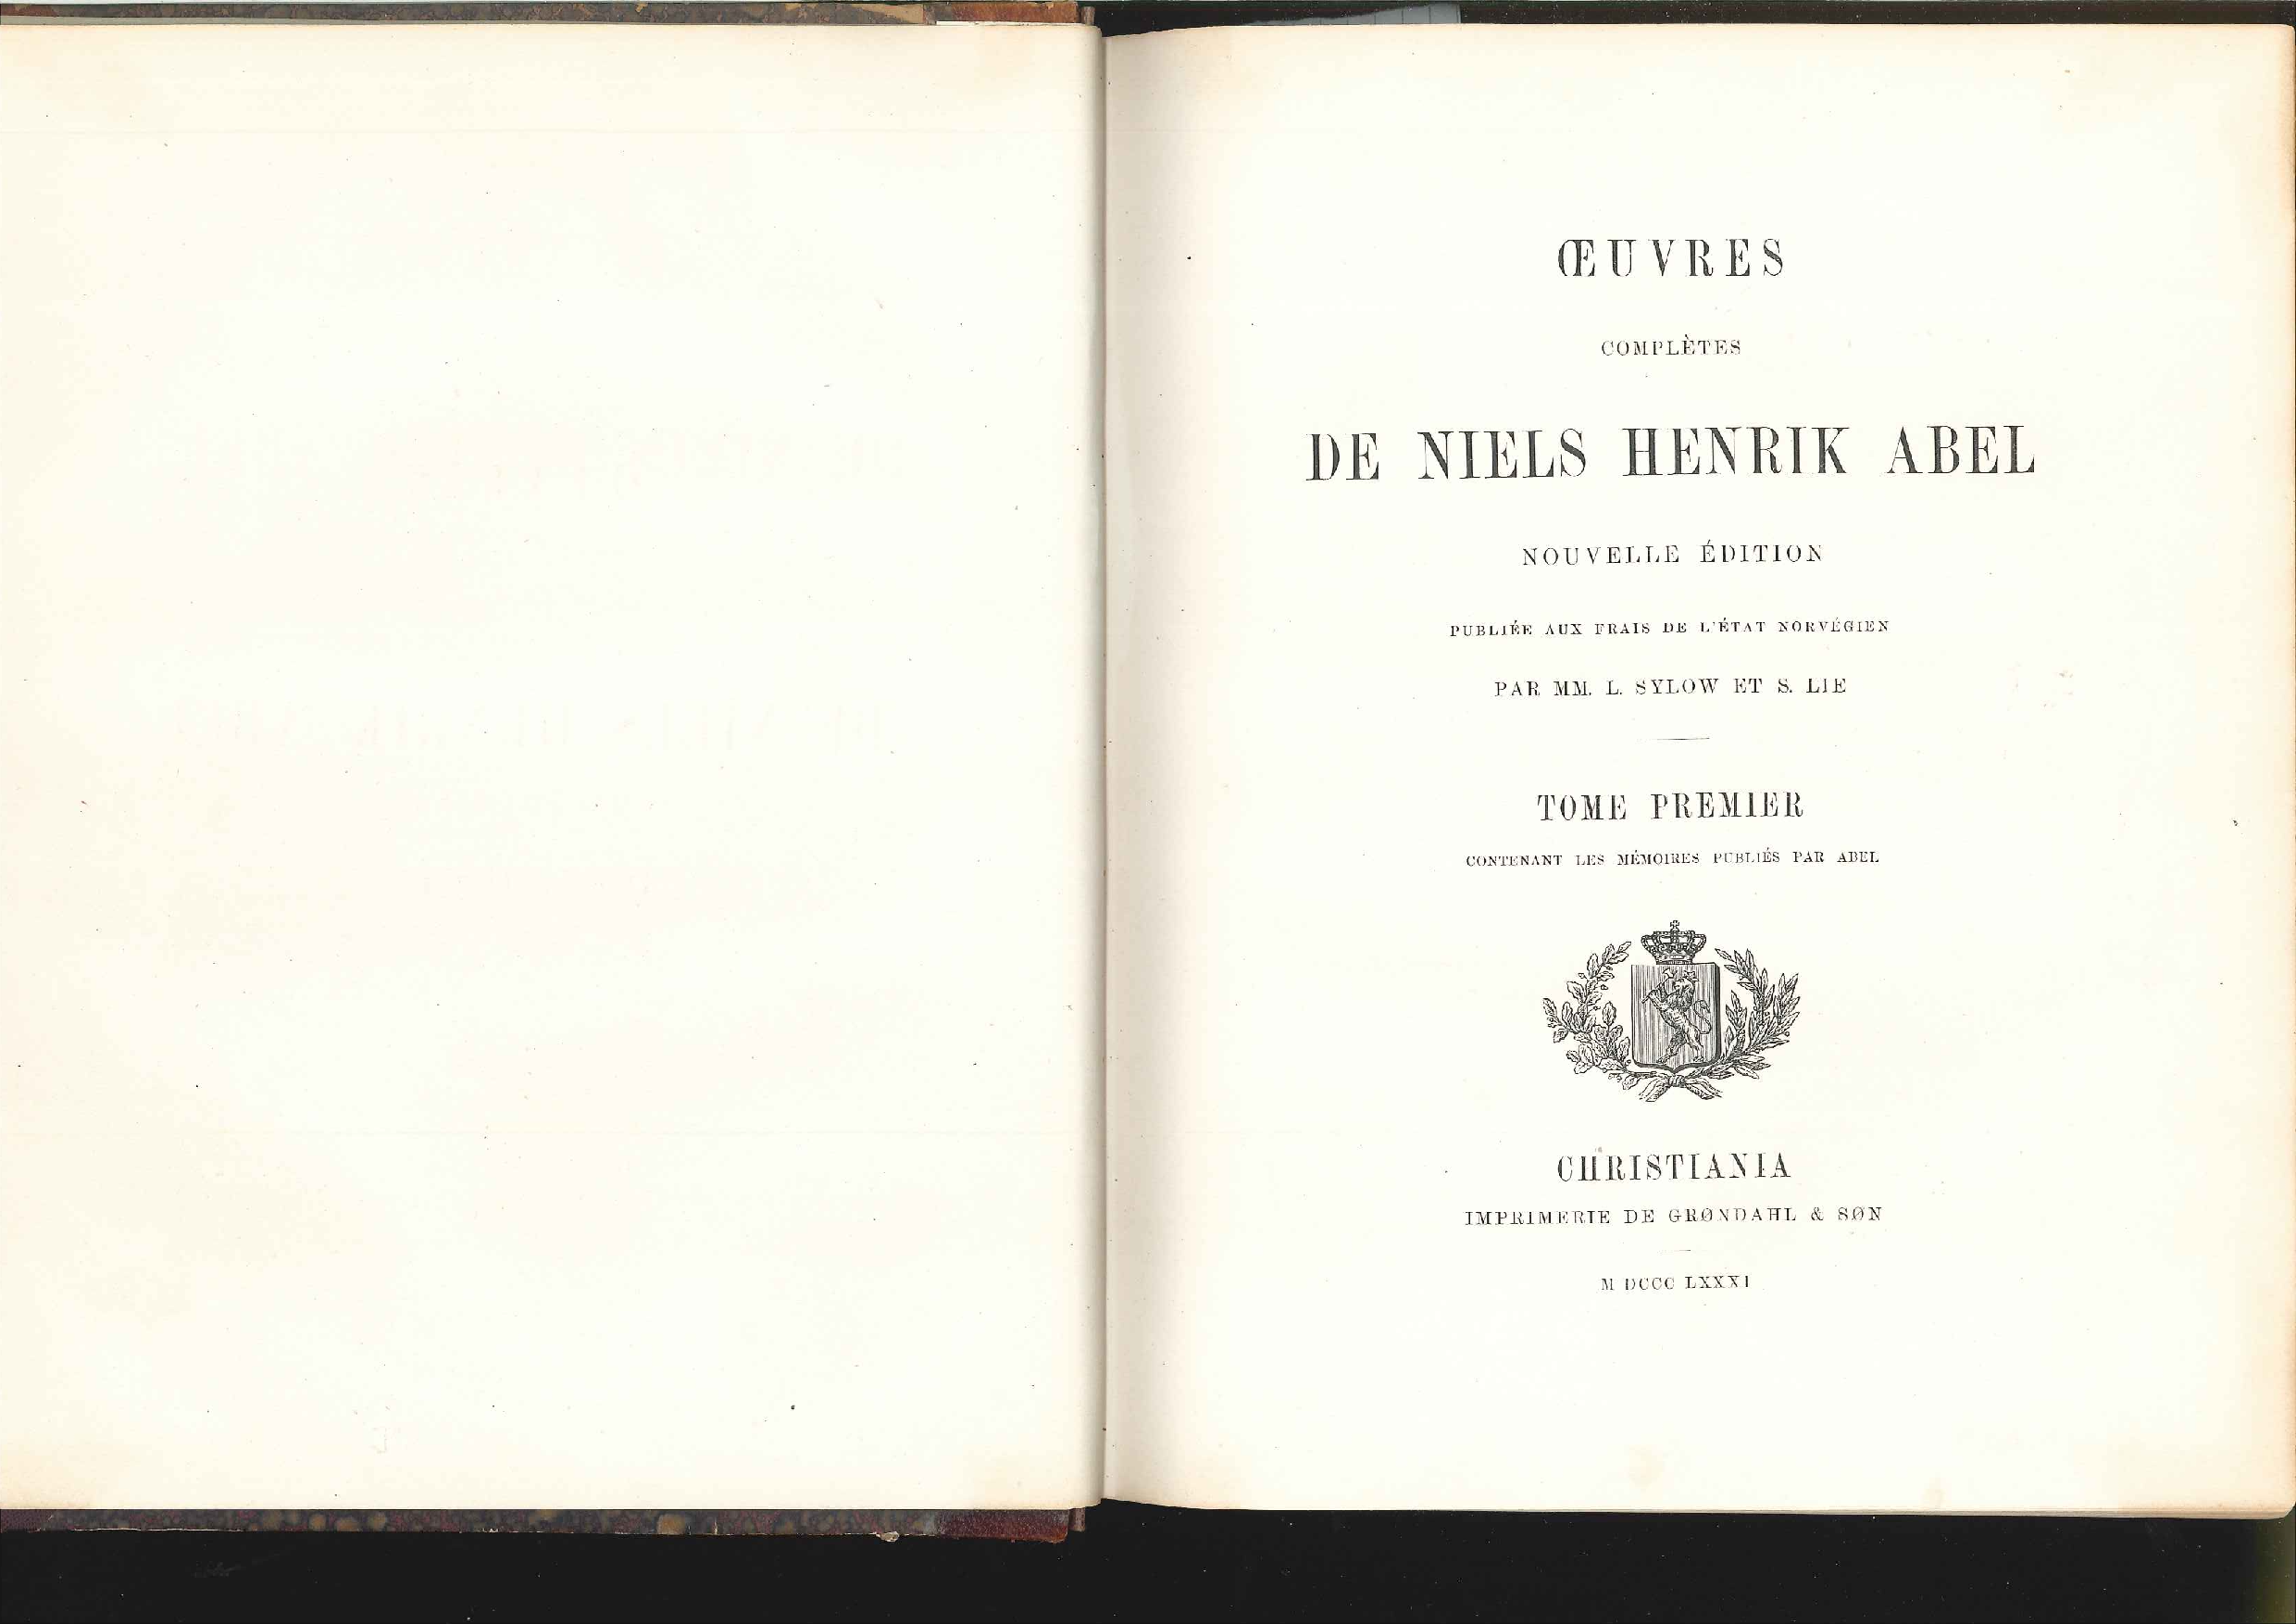
\includepdf[pages={1-4},nup=1x2,templatesize={\linewidth}{0.65\linewidth},landscape=false,offset=0mm 0mm,delta=2mm 2mm
,addtotoc={1,section,1,{\em R\'esolution du'un probl\`eme de mechanique by Niels Henrik Abel},ORIGINALResolutionOfAMechanicalProblemByNielsHenrikAbel}
]{figures/20160720AbelTransformOriginal.pdf}
%\begin{figure}
% \centering 
% 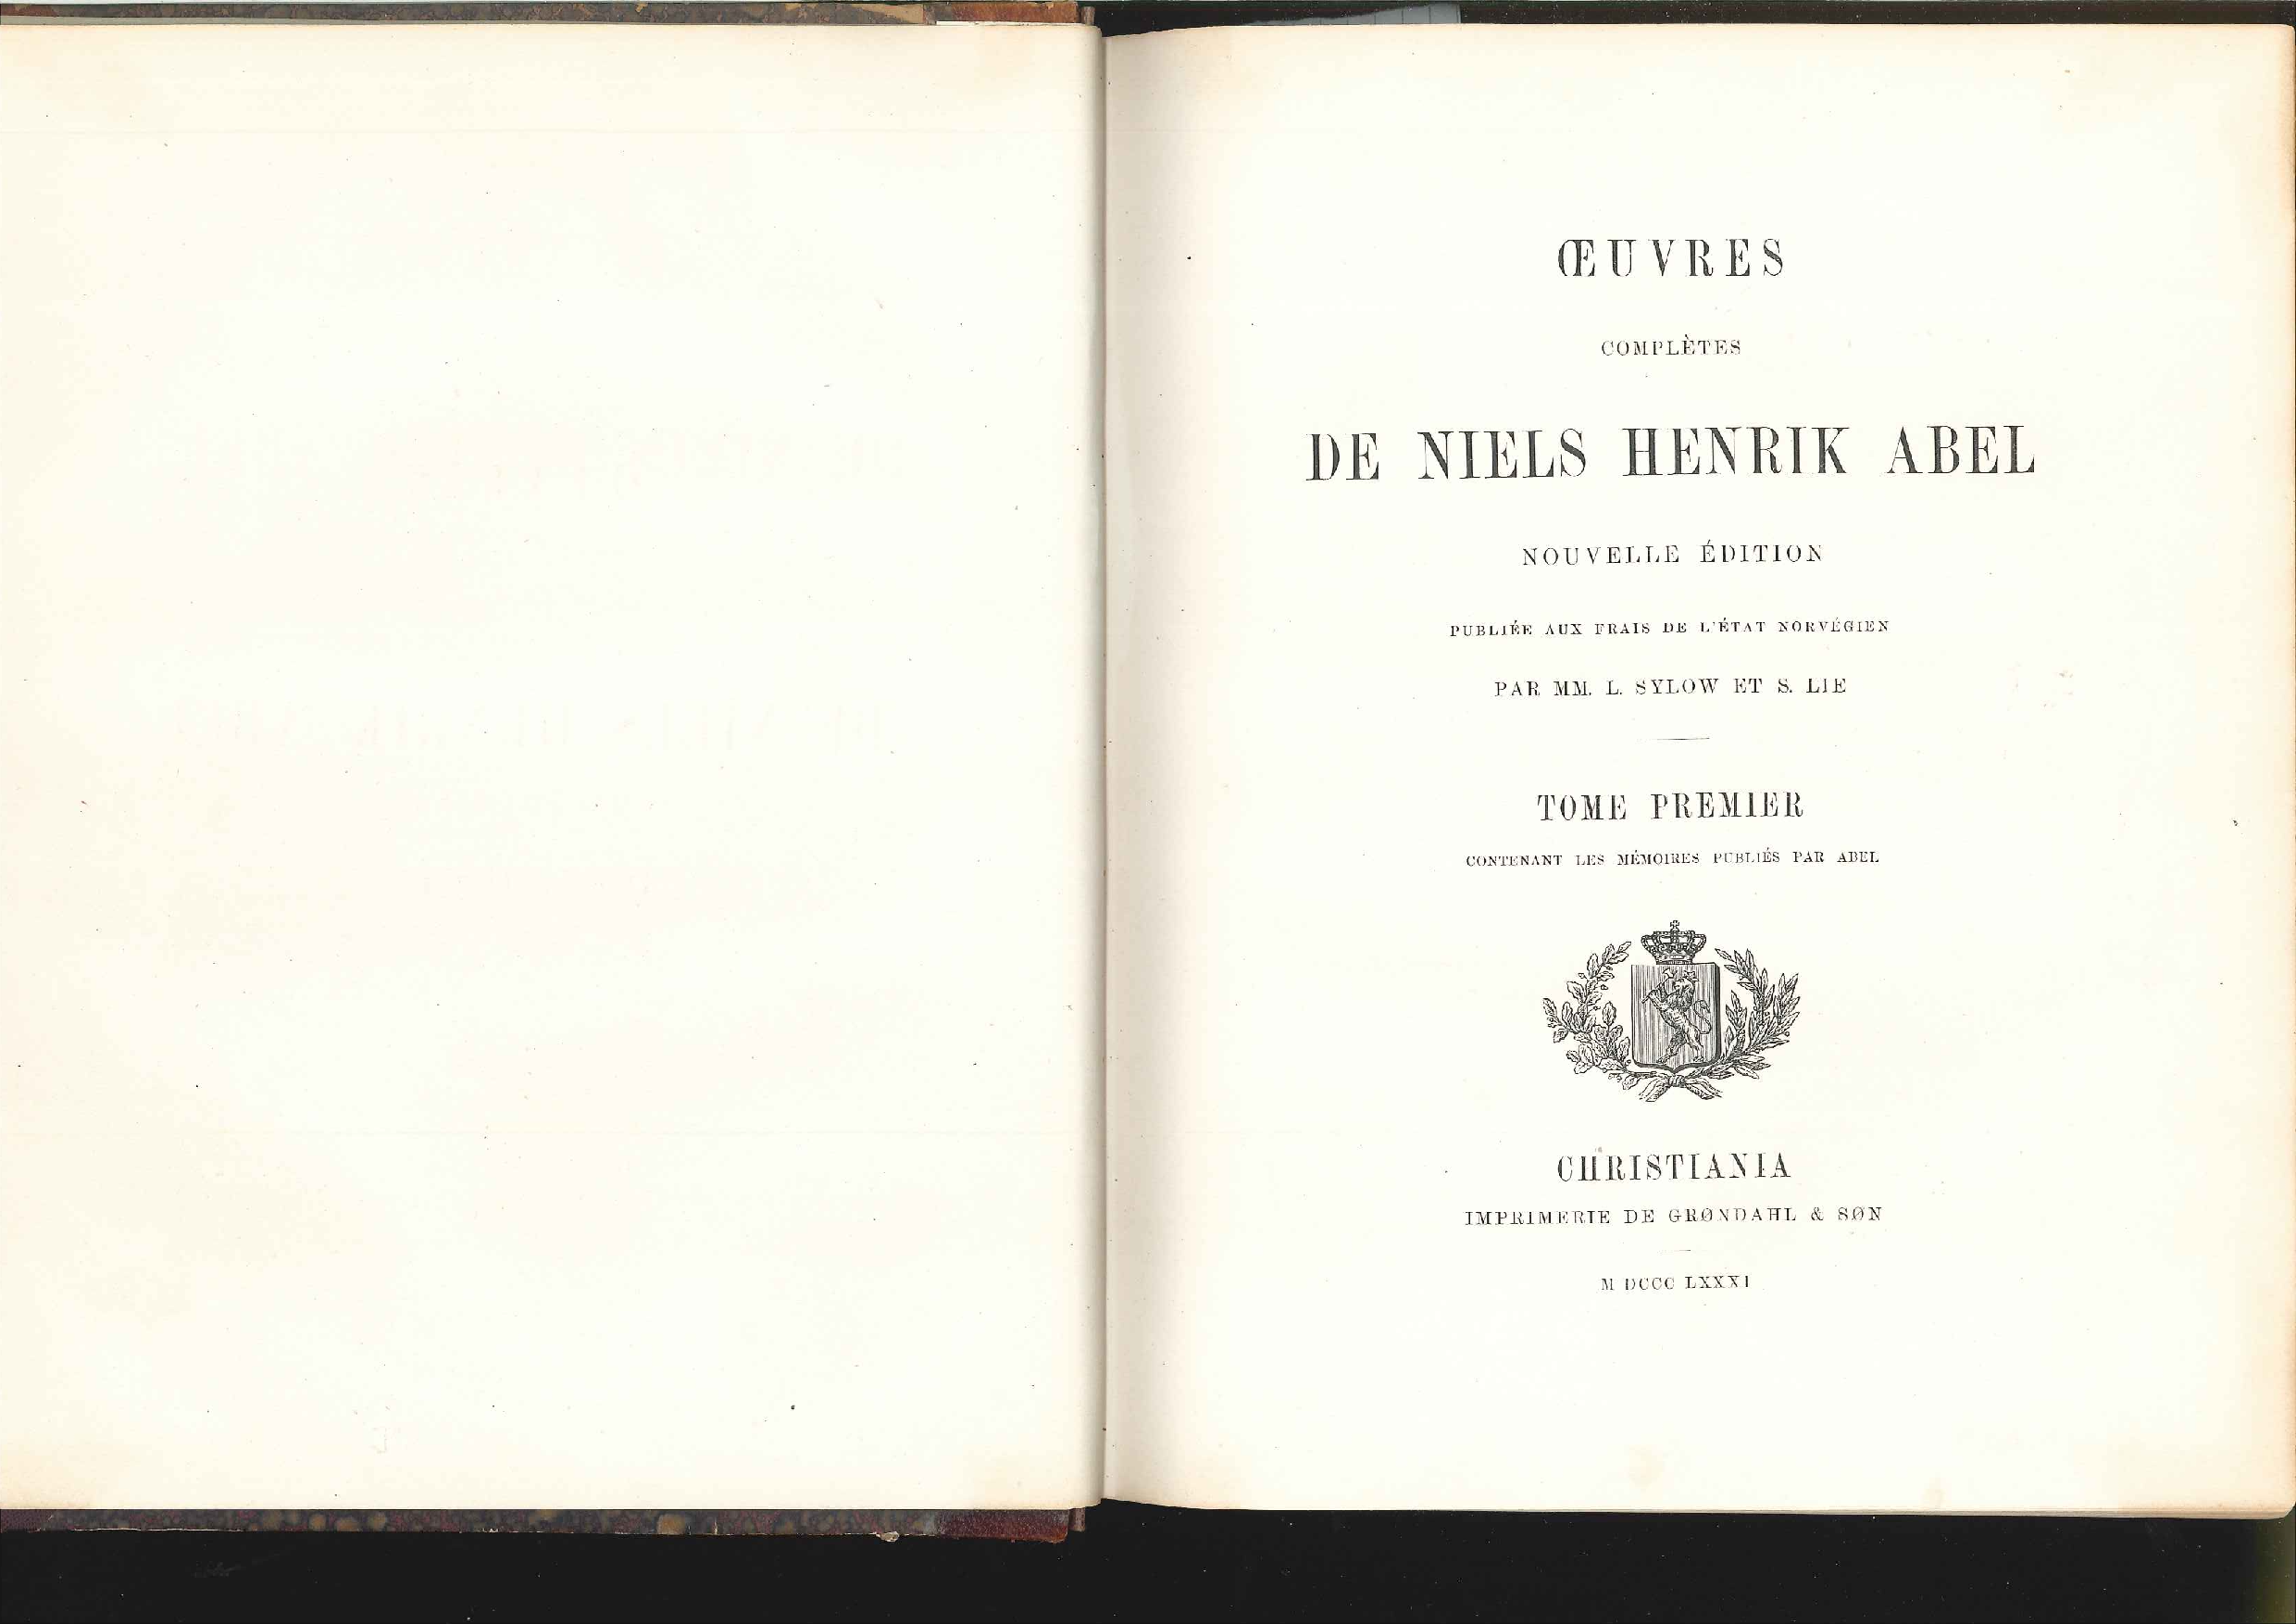
\includegraphics{figures/20160720AbelTransformOriginal.pdf}
%\end{figure}

%%%%%%%%%%%%%%%%%%%%%%%%  ENDING   OF  CHAPTER %%%%%%%%%%%%%%%%%%%%%%%%%%%%%%%%


%%%%%%%%%%%%%%%%%%%%%%%%  BEGINNING OF CHAPTER %%%%%%%%%%%%%%%%%%%%%%%%%%%%%%%%
\chapter{Lagrange's Equations of Motion}

We give a brief exposition of Lagrange's equation of motion (1788) that builds on Newton's insights.

\emph{Recommended Recollections:} Mechanical work\footnote{\url{https://en.wikipedia.org/wiki/Work_(physics)}} is the 
dot-product\footnote{\url{https://en.wikipedia.org/wiki/Dot_product}} of 
force\footnote{\url{https://en.wikipedia.org/wiki/Force}} 
and displacement\footnote{\url{https://en.wikipedia.org/wiki/Displacement_(vector)}}.
Other basic ideas we will use include: (i) the chain rule of claculus\footnote{\url{https://en.wikipedia.org/wiki/Chain_rule}}, (ii) pythogorean theorem\footnote{\url{https://en.wikipedia.org/wiki/Pythagorean_theorem}}, (iii) trigonometric functions\footnote{\url{https://en.wikipedia.org/wiki/Trigonometric_functions}}, (iv) arc-geometry\footnote{\url{https://en.wikipedia.org/wiki/Arc_(geometry)}}, (v) arc-length\footnote{\url{https://en.wikipedia.org/wiki/Arc_length}}, ... %\footnote{\url{}}

\section{The role of kinetic energy}

\subsection{Phase and position of a particle}
Given $k$ degrees of freedom for a moving or dynamic particle (idealized mass-point) let its state in this phases space $\Rz^k$ be 
\[
\theta : =\left( \theta_1,\theta_2,\ldots,\theta_k\right), \quad k \in \Nz:=\{1,2,3,\ldots\}, k < \infty.
\]
Let $p$ be a vector-valued twice-continuously differentiable function of $\theta$ that maps a phase $\theta \in \Rz^k$ into a position $p(\theta) \in \Rz^3$:
\[
C^2 \ni p := p(\theta) := p(\theta_1,\theta_2,\ldots,\theta_k), \quad \Rz^k \ni p(\theta) \mapsto (x,y,z) \in \Rz^3.
\]
Recall that $C^2 \ni p(\theta)$ means that the following derivatives are well-defined:
\[
\frac{\dd p}{\dd \theta_i} = \frac{\dd p(\theta_1,\theta_2,\ldots,\theta_k)}{\dd \theta_i} \quad \forall i \in [k]:=\{1,2,\ldots,k\},
\]
and the following mixed derivatives are well-defined:
\[
\frac{\dd p}{\dd \theta_i \dd \theta_j} = \frac{\dd p(\theta_1,\theta_2,\ldots,\theta_k)}{\dd \theta_i \dd \theta_j} \quad \forall (i,j) \in [k]^2 := [k]\times[k].
\]
\subsection{Time and dynamics}
Now let $t \in [0,\infty) \subset \Rz$ denote the time since the beginning of observation at $t=0$.  
If we are given $k$ time-dependent functions in the phase space:
\[
t \mapsto \theta(t) = \left( \theta_1(t),\theta_2(t),\ldots,\theta_k(t)\right),
\]
then the map $t \mapsto p(\theta(t))$ {\em moves} the position of the particle in $\Rz^3$ through time $t$:
\[
[0,\infty) \ni t \mapsto p(\theta(t)) = p\left( \theta_1(t),\theta_2(t),\ldots,\theta_k(t)\right) = \left( x(t), y(t), z(t) \right) \in \Rz^3.
\]

\subsection{Chain rule gives the velocity and acceleration vectors}
{\em Velocity} is the rate of change of the particle's position with respect to time.  
By the chain rule of calculus, the velocity of the particle is:
\begin{align*}
\dot{p} 
&:= \frac{\dd p}{\dd t} := \frac{\dd p(\theta(t))}{\dd t} := \frac{\dd p(\theta_1(t),\theta_2(t),\ldots,\theta_k(t))}{\dd t} \\
&= \sum_{i=1}^k \frac{\dd p(\theta_1(t),\theta_2(t),\ldots,\theta_i(t),\ldots,\theta_k(t))}{\dd \theta_i(t)} \times \frac{\dd \theta_i(t)}{\dd t}\\
&=: \sum_{i=1}^k \frac{\dd p}{\dd \theta_i} \dot{\theta_i}.
\end{align*}
Acceleration is the rate of change of the particle's velocity with respect to time.  
By the chain rule of calculus, the acceleration of the particle is:
\begin{align*}
\ddot{p} 
&:= \frac{\dd }{\dd t}\left(\frac{\dd p}{\dd t}\right)\\
&~\\
&= ..\\
&~\\
&= ..\\
&~\\
&= ..\\
&~\\
&= ..\\
&~\\
&=: \sum_{i=1}^k \sum_{j=1}^k \frac{\dd ^2 p}{\dd \theta_i \dd \theta_j} \dot{\theta_i}\dot{\theta_j}
  + \sum_{i=1}^k \frac{\dd p}{\dd \theta_i} \ddot{\theta_i}.
\end{align*} 

\subsection{The kinetic energy}
Say, $t$ is fixed and the particle has $1$ unit of mass $m$.  
Then the {\em kinetic energy} is given by:
\begin{align*}
\Tc 
&:= 
\frac{1}{2} \eN{\dot{p}}^2 = \frac{1}{2} \sqrt{\sum_{i=1}^k \left( \frac{\dd p}{\dd t}\right)^2}\\
&~\\
&= ..\\
&~\\
&= ..\\
&~\\
&= ..\\
&~\\
&= ..\\
&~\\
&= \frac{1}{2} \sum_{i=1}^k \sum_{j=1}^k \dP{\frac{\dd p}{\dd \theta_i}(t),\frac{\dd p}{\dd \theta_j(t)}} \dot{\theta}_i(t) \dot{\theta}_j(t)\\
&=: \frac{1}{2} \sum_{i=1}^k \sum_{j=1}^k \dP{\frac{\dd p}{\dd \theta_i},\frac{\dd p}{\dd \theta_j}} \dot{\theta}_i \dot{\theta}_j
\end{align*}
Now regard $\Tc$ as a function of $t$-specific $k$-tuples $\theta(t)$ and $\dot{\theta}(t)$:
\[
(\theta(t),\dot{\theta}(t)) \mapsto \Tc(\theta(t),\dot{\theta}(t))
\] 
Then for each fixed $i \in [k]$, by calculus:
\[
\frac{\dd \Tc}{\dd \dot{\theta}_i} = \sum_{j=1}^k \dP{ \frac{\dd p}{\dd \theta_i},\frac{\dd p}{\dd \theta_j}} \dot{\theta}_j
\]
and
\[
\frac{\dd \Tc}{\dd {\theta}_i} = \sum_{\ell=1}^k \sum_{j=1}^k \dP{ \frac{\dd^2 p}{\dd \theta_{\ell} \dd \theta_j}, \frac{\dd p}{\dd \theta_j} } \dot{\theta}_{\ell} \theta_j.
\]
Notice the factor of $1/2$ disappears from the fact that $\dP{\cdot}$ is summetric.

\subsection{The Lagrangian}
For each fixed $i \in [k]$:
\[
\Lc_i := \frac{\dd}{\dd t} \left( \frac{\dd \Tc}{\dd \dot{\theta}_i} \right) - \frac{\dd \Tc}{\dd \theta_i}
\]
The theorem fround by calculus is:
\[
\Lc_i = \dP{ \frac{\dd p}{\dd \theta_i}, \ddot{p} }
\]
This is fundamental via Newton! whereby
for small displacement $\delta \theta_i$ at any time $t$ we have the corresponding change in position given by:
\[
\delta p \approxeq \frac{\dd p}{\dd \theta_i} \cdot \delta \theta_i .
\]

\subsection{Following Newton's infinitesimal work}
The basic idea is to follow newton's infinitesimal work!  
By Newton the work to displace the particla from point $p$ to the point $p + \delta p$ is
\[
\pm m \dP{dp, \ddot{p}}  = \underset{\text{scale-factor for work}}{\underbrace{\dP{\frac{\dd p}{\dd \theta_i}{\ddot{p}}}}}\cdot \delta \theta_i, \quad
\text{when } \theta_i \mapsto \theta_i + \delta \theta_i
\]
In the special case where the external force is a potential
\[
\Uc := \Uc (\theta) := \Uc \left( (\theta_1,\theta_2,\ldots,\theta_k) \right)
\]
then this infinitesimal work is 
\[
\pm \frac{\dd \Uc}{\dd \theta_i} \implies \Lc_i = \pm \frac{\dd \Uc}{\dd \theta_i}
\]
The sign is understood for the specific problem at hand via by examples.
\section{Example: a simple pendulum}


%%%%%%%%%%%%%%%%%%%%%%%%  ENDING   OF  CHAPTER %%%%%%%%%%%%%%%%%%%%%%%%%%%%%%%%


%%%%%%%%%%%%%%%%%%%%%%%%  BEGINNING OF CHAPTER %%%%%%%%%%%%%%%%%%%%%%%%%%%%%%%%
\chapter{Linear Algebra}
%%%%%%%%%%%%%%%%%%%%%%%%  ENDING   OF  CHAPTER %%%%%%%%%%%%%%%%%%%%%%%%%%%%%%%%


%%%%%%%%%%%%%%%%%%%%%%%%  BEGINNING OF CHAPTER %%%%%%%%%%%%%%%%%%%%%%%%%%%%%%%%
\chapter{Stokes theorem}
%%%%%%%%%%%%%%%%%%%%%%%%  ENDING   OF  CHAPTER %%%%%%%%%%%%%%%%%%%%%%%%%%%%%%%%


%%%%%%%%%%%%%%%%%%%%%%%%  BEGINNING OF CHAPTER %%%%%%%%%%%%%%%%%%%%%%%%%%%%%%%%
\chapter{Measures}
%%%%%%%%%%%%%%%%%%%%%%%%  ENDING   OF  CHAPTER %%%%%%%%%%%%%%%%%%%%%%%%%%%%%%%%


%%%%%%%%%%%%%%%%%%%%%%%%  BEGINNING OF CHAPTER %%%%%%%%%%%%%%%%%%%%%%%%%%%%%%%%
%\chapter{}
%%%%%%%%%%%%%%%%%%%%%%%%  ENDING   OF  CHAPTER %%%%%%%%%%%%%%%%%%%%%%%%%%%%%%%%

%%%%%%%%%%%%%%%%%%%%%%%%  END OF BOOK  %%%%%%%%%%%%%%%%%%%%%%%%%%%%%%%%%%%%%%%%
%%%%%%%%%%%%%%%%%%%%%%%%%%%%%%%%%%%%%%%%%%%%%%%%%%%%%%%%%%%%%%%%%%%%%%%%%%%%%%%
\end{document}
